\documentclass[12pt]{article}

% ── Packages ──────────────────────────────────────────────────────────────────
\usepackage[margin=1in]{geometry}
\usepackage{amsmath,amssymb,amsthm}
\usepackage{graphicx}
\usepackage{booktabs}
\usepackage{hyperref}
\usepackage{natbib}
\usepackage{setspace}
\usepackage{microtype}
\usepackage{xcolor}
\usepackage{enumitem}
\usepackage{caption}
\usepackage{subcaption}
\usepackage{array}
\usepackage{multirow}
\usepackage{float}
\usepackage{url}
\usepackage{mathtools}

% ── Hyperref setup ────────────────────────────────────────────────────────────
\hypersetup{
  colorlinks=true,
  linkcolor=blue!70!black,
  citecolor=blue!70!black,
  urlcolor=blue!70!black
}

% ── Spacing ───────────────────────────────────────────────────────────────────
\onehalfspacing

% ── Custom commands ───────────────────────────────────────────────────────────
\newcommand{\pfill}{\hat{P}_{\mathrm{fill}}}
\newcommand{\Fhat}{\hat{F}}
\newcommand{\Shat}{\hat{S}}
\newcommand{\given}{\,|\,}

% ── Title block ───────────────────────────────────────────────────────────────
\title{
  \textbf{Latency-Compensating Market Making:}\\[4pt]
  \textbf{An AI Framework for Retail Liquidity Provision}\\[10pt]
  \large Version 1.8 --- Working Paper
}

\author{
  Jude Kriel Ramcharitar\\[4pt]
  \small Independent Researcher\\
  \small \href{mailto:j.k.ramcharitar@gmail.com}{j.k.ramcharitar@gmail.com}\\
  \small ORCID: 0009-0004-8190-1958
}

\date{June 2026}

% ══════════════════════════════════════════════════════════════════════════════
\begin{document}
\maketitle
\thispagestyle{empty}

% ── Abstract ──────────────────────────────────────────────────────────────────
\begin{abstract}
High-frequency market makers profit by being faster than everyone else --- co-located servers, microwave links, and fiber routes optimized to the millisecond. For retail traders and non-institutional algorithms operating under execution delays of 200 milliseconds to 2 seconds, participating in market making has been effectively impossible: by the time a quote is submitted, the market has already moved, and the slow trader absorbs the loss. This latency gap is not merely a competitive disadvantage --- it is a structural barrier that concentrates a recurring and significant source of financial returns among a small number of technologically privileged firms. Proposed market design reforms, including speed bumps and frequent batch auctions, address this asymmetry at the exchange level but remain unadopted at scale and offer no recourse to the individual participant. This paper proposes \emph{latency-compensating market making}: an AI-driven framework in which predictive models trained on limit order book microstructure data substitute for execution speed by anticipating market conditions within the trader's latency window. We develop a two-component system --- a deep learning fill probability estimator using survival analysis, and a latency-aware reinforcement learning agent for dynamic quote optimization --- and formalize the conditions under which prediction-based compensation is theoretically viable. We outline an empirical research agenda targeting cryptocurrency markets, where retail participation in liquidity provision is structurally accessible, and position this framework as a contribution to the broader question of how artificial intelligence can reduce structural inequities in market access. This work connects market microstructure theory, machine learning methodology, and financial regulation, with direct implications for policymakers designing equitable market infrastructure and for the growing population of retail algorithmic traders seeking meaningful participation in modern financial markets.
\end{abstract}

\newpage
\tableofcontents
\newpage

% ══════════════════════════════════════════════════════════════════════════════
\section{Introduction}
% ══════════════════════════════════════════════════════════════════════════════

In competitive markets, speed is capital. The firms that dominate modern equity and cryptocurrency liquidity provision have spent billions of dollars compressing their execution latency to microseconds --- not because microseconds matter to the economy, but because being first to respond to a price signal is worth money, every time, at scale. This raises a question that is both intellectually precise and practically urgent: \textbf{is speed itself the valuable resource, or is it merely a proxy for something more fundamental --- the ability to act on information before it becomes stale?}

If the answer is the latter, then speed may not be strictly necessary. A market participant who cannot act in microseconds might still act \emph{correctly} --- if they can predict, with sufficient accuracy, what the market will look like when their order arrives. This paper pursues that hypothesis. We propose that artificial intelligence, specifically deep learning models trained on limit order book microstructure data, can serve as a latency compensation mechanism: substituting predictive accuracy for execution speed in the market making problem.

The practical motivation is significant. Market making --- the continuous posting of bid and ask limit orders to earn the bid-ask spread --- is one of the few systematic, non-directional strategies available to algorithmic traders. Institutional market makers generate consistent returns by providing liquidity and managing inventory risk. Yet retail and non-institutional traders operating under execution delays of 200 milliseconds to 2 seconds are effectively excluded from this activity. Under standard market making frameworks derived from the foundational work of \citet{avellaneda2008}, a trader who cannot cancel and repost quotes faster than adverse price movements accumulates toxic inventory and generates negative expected returns. Latency is not merely an inconvenience --- it is a structural exclusion mechanism.

Existing responses to this problem operate at the wrong level. Proposed market design reforms --- including the IEX speed bump \citep{hu2019}, frequent batch auctions \citep{budish2015}, and micro-burst fees \citep{brolley2023} --- address latency asymmetry at the exchange level. They require regulatory adoption, exchange cooperation, and in most cases have seen limited real-world implementation. They offer nothing to the individual trader operating today, on existing infrastructure, in existing markets. The reinforcement learning market making literature \citep{spooner2018,guo2023} has produced sophisticated quoting agents but uniformly assumes low-latency execution environments. The most directly relevant recent work, RELAVER \citep{jiang2025}, explicitly models execution delays but targets a 30--100 millisecond regime --- still an order of magnitude faster than the retail execution environment we consider.

This paper makes four contributions. First, we formally define the latency-compensating market making problem, characterizing the conditions under which predictive models can offset execution delay costs. Second, we propose a deep survival analysis model for fill probability estimation in the limit order book, extending the convolutional-transformer architecture of \citet{arroyo2024} to explicitly condition on a configurable latency window. Third, we develop a latency-aware reinforcement learning agent that integrates fill probability predictions and short-term price direction signals into a unified quoting policy optimized for retail-scale execution delays. Fourth, we outline an empirical research agenda using cryptocurrency limit order book data, where retail participation in liquidity provision is structurally accessible and high-quality data is publicly available.

The broader implication of this work extends beyond trading strategy. If predictive compensation for latency disadvantage is viable --- even partially --- it suggests that artificial intelligence may serve as a genuine democratizing force in market microstructure, reducing the structural concentration of liquidity provision returns among technologically privileged institutions.

The remainder of this paper is organized as follows. Section~\ref{sec:lit} reviews the relevant literature. Section~\ref{sec:formalization} formalizes the latency-compensating market making problem. Section~\ref{sec:fillmodel} describes the fill probability model. Section~\ref{sec:rl} presents the reinforcement learning framework. Section~\ref{sec:empirical} outlines the empirical research agenda. Section~\ref{sec:policy} discusses policy implications and Section~\ref{sec:conclusion} concludes.

% ══════════════════════════════════════════════════════════════════════════════
\section{Literature Review}
\label{sec:lit}
% ══════════════════════════════════════════════════════════════════════════════

This paper sits at the intersection of four bodies of literature: market making theory, the economics of latency and high-frequency trading, deep learning models for limit order book prediction, and reinforcement learning for algorithmic trading. We review each in turn, identifying the cumulative gap that motivates our contribution.

\subsection{Market Making Theory}

The modern theoretical framework for market making originates with the inventory-based models of \citet{garman1976} and \citet{ho1981}, which characterized the market maker's problem as one of simultaneously managing spread revenue and inventory risk. The seminal contribution of \citet{avellaneda2008} formalized this as a stochastic optimal control problem, deriving closed-form expressions for optimal bid and ask quotes as a function of inventory position, risk aversion, and order arrival intensity. This framework remains the dominant analytical foundation for market making research and the baseline against which new approaches are benchmarked.

Subsequent work extended the Avellaneda-Stoikov framework in several directions. Cartea, Jaimungal and colleagues developed a series of models incorporating adverse selection, alpha signals, and execution uncertainty into the optimal control formulation \citep{cartea2018}. \citet{cartea2023} introduced stochastic delay into the optimal execution problem, providing one of the first formal treatments of latency as a structural risk factor rather than a background assumption.

A critical limitation shared by virtually all analytical market making models is the implicit assumption of negligible or symmetric execution latency. As \citet{lehalle2022} demonstrate formally, this assumption is not merely a simplification --- it is load-bearing. They show that the value of predictive signals about future order flow is systematically eroded by latency: a trader who can predict adverse flow but cannot act on that prediction fast enough derives diminishing benefit from the signal. This finding identifies precisely the problem our framework addresses, and motivates the shift from reactive to predictive quoting that we propose.

\subsection{Latency, High-Frequency Trading, and the Arms Race}

The economics of latency in financial markets have been extensively studied since the proliferation of electronic trading in the early 2000s. \citet{moallemi2013} provided the first formal theoretical model of latency cost for a representative investor, showing that median latency costs for NYSE common stocks roughly tripled between 1995 and 2005 as markets electronified.

The competitive dynamics of latency investment were characterized as an arms race by \citet{budish2015}, whose influential theoretical work argued that continuous-time limit order book markets create structural incentives for socially wasteful speed investment. \citet{aquilina2022} provided landmark empirical quantification of this phenomenon, finding that latency arbitrage races occur approximately once per minute per symbol for FTSE 100 stocks, with modal race durations of 5--10 microseconds. Their estimate that eliminating latency arbitrage through frequent batch auctions would reduce effective spreads by approximately 17\% provides a precise measure of the ongoing tax that speed asymmetry imposes on slower market participants.

The structural disadvantage faced by retail participants has been documented empirically by several studies. Research shows that high-frequency trading firms account for 50--60\% of U.S.\ equity trading volume \citep{lin2024}, and that retail investors underperform institutional benchmarks systematically. Proposed solutions including the IEX speed bump \citep{hu2019}, frequent batch auctions \citep{budish2015}, micro-burst fees \citep{brolley2023}, and the Lorentz-Invariant Auction mechanism \citep{barzykin2026} represent market design responses to latency asymmetry. While theoretically promising, these interventions require exchange-level adoption and regulatory coordination that has thus far limited their real-world impact. Critically, none offers recourse to the individual trader operating within existing market infrastructure --- the population this paper directly addresses.

A separate and emerging concern is the risk of algorithmic collusion among AI-powered trading systems. \citet{dou2025} demonstrate that reinforcement learning trading agents can autonomously sustain collusive supra-competitive profits without explicit coordination, through two distinct mechanisms they term price-trigger strategies and homogenized learning biases. This finding motivates the policy discussion in Section~\ref{sec:policy} regarding the regulatory implications of democratized AI market making.

\subsection{Limit Order Book Prediction and Fill Probability Estimation}

A substantial machine learning literature has developed around the prediction of short-term price movements and order execution outcomes from limit order book data. Early deep learning approaches, notably DeepLOB \citep{zhang2019}, established that convolutional neural networks could extract predictive features from the spatial structure of the order book. Subsequent architectures incorporated attention mechanisms and transformer designs to capture longer-range temporal dependencies in order flow \citep{jung2024,berti2025}.

The specific problem of fill probability estimation --- predicting whether and when a limit order posted at a given price level will execute --- has received targeted attention more recently. \citet{lo2002} established early econometric foundations for execution probability modeling. \citet{maglaras2022} introduced the first deep learning approach to fill probability estimation. \citet{arroyo2024} significantly advanced this line of work with a convolutional-transformer architecture incorporating survival analysis --- a statistical framework naturally suited to the right-censored nature of limit order fill data. Most recently, the KANFormer architecture \citep{kanformer2024} has proposed improvements in interpretability and evaluation protocol over the \citeauthor{arroyo2024} baseline.

Our specific contribution relative to existing work is the explicit conditioning of fill probability estimates on a configurable latency window $\ell$ --- the delay between the trader's quoting decision and the order's arrival at the exchange. Existing models estimate fill probabilities from the perspective of an order already resting in the book; we require estimates from the perspective of an order not yet submitted, accounting for the market state change that will occur during transmission.

\subsection{Reinforcement Learning for Market Making}

The application of reinforcement learning to market making has emerged as a productive research direction over the past decade. \citet{spooner2018} provided an early demonstration that RL agents could learn competitive market making policies through interaction with simulated order book environments. \citet{guo2023} introduced continuous action spaces and attention-based LOB feature extraction, improving the practical applicability of RL market makers to realistic quote granularity. \citet{briola2021} demonstrated RL-based market making in high-frequency cryptocurrency settings.

A persistent limitation of this literature is the treatment of execution as instantaneous or near-instantaneous. The most direct treatment of this gap is the recent RELAVER framework \citep{jiang2025}, which builds a realistic market making environment with random execution delays of 30--100 milliseconds. Our work extends this frontier: RELAVER addresses institutional-grade latency (30--100ms); we target the retail latency regime (200ms--2s), which is an order of magnitude larger and introduces qualitatively different challenges.

\subsection{Positioning This Work}

Latency-compensating market making, as we define and develop it here, occupies the intersection of all four bodies of literature reviewed above --- and to our knowledge, no existing work has pursued this specific formulation.

% ══════════════════════════════════════════════════════════════════════════════
\section{Problem Formalization}
\label{sec:formalization}
% ══════════════════════════════════════════════════════════════════════════════

We formalize the latency-compensating market making problem by extending the classical Avellaneda-Stoikov framework to explicitly incorporate execution delay as a structural risk factor, and by introducing the role of predictive models in compensating for that delay.

\subsection{The Standard Market Making Setup}

Consider a market maker operating over a finite time horizon $[0, T]$. The mid-price of the asset follows a standard Brownian motion:
\begin{equation}
  S_t = S_0 + \sigma W_t,
\end{equation}
where $\sigma > 0$ is the asset volatility and $W_t$ is a standard Brownian motion. The market maker posts bid and ask limit orders at offsets $\delta_b$ and $\delta_a$ from the mid-price. Following \citet{avellaneda2008}, the resulting order arrival rates decay exponentially with quote offset:
\begin{equation}
  \lambda_b(\delta_b) = A \cdot e^{-k\delta_b}, \qquad
  \lambda_a(\delta_a) = A \cdot e^{-k\delta_a},
\end{equation}
where $A > 0$ and $k > 0$ are market parameters. The market maker's inventory $q_t$ evolves as fills arrive on each side, and their wealth $X_t$ accumulates from spread capture net of inventory risk. The objective is to maximize expected terminal utility:
\begin{equation}
  \max_{\delta_b,\, \delta_a} \;\mathbb{E}\bigl[X_T + q_T S_T - \gamma q_T^2\bigr],
\end{equation}
where $\gamma > 0$ is the inventory risk aversion parameter penalizing large terminal positions.

\subsection{Introducing Execution Latency}

We depart from the standard framework by introducing execution latency $\ell$, defined as the round-trip delay between the agent's quoting decision and the order's insertion into the exchange order book:
\begin{equation}
  \ell \in [200\,\text{ms},\; 2000\,\text{ms}],
\end{equation}
characterizing the execution environment of retail and non-institutional algorithmic traders operating without co-location infrastructure.

Under latency $\ell$, the fill probability for a quote at offset $\delta$ depends not on the current market state $\mathcal{F}_t$ but on the market state at the time of order arrival, $\mathcal{F}_{t+\ell}$, which is unobserved at the time of the quoting decision:
\begin{equation}
  P_{\mathrm{fill}}(\delta,\, \ell,\, \mathcal{F}_{t+\ell}) = \mathbb{P}\bigl[\text{order fills} \given \delta,\, \mathcal{F}_{t+\ell}\bigr].
\end{equation}
Since $\mathcal{F}_{t+\ell}$ is unknown at quoting time, the market maker must estimate it using a predictive model, denoted $\hat{\mathcal{F}}_{t+\ell}$.

This creates two compounding sources of loss relative to the zero-latency benchmark:

\paragraph{Adverse selection amplification.} If the mid-price moves adversely by more than $\delta$ during the latency window, the market maker is filled at a stale price and immediately holds a losing position. The expected loss per adverse fill grows with $\ell$ because larger latency windows permit more mid-price drift before the order arrives.

\paragraph{Cancellation impotence.} In the standard model, a market maker who detects an adverse signal can cancel their quote before being filled. Under latency $\ell$, any cancellation instruction takes $\ell$ milliseconds to reach the exchange. The fill may already have occurred by the time the cancel arrives, making the cancellation option effectively worthless during fast adverse moves.

\subsection{The Latency-Compensating Market Making Problem}

We define the latency-compensating market making problem as the optimization of quoting decisions under latency $\ell$, using a predictive estimate $\hat{\mathcal{F}}_{t+\ell}$ of the future market state in place of the unobservable true state $\mathcal{F}_{t+\ell}$.

Formally, let $\pfill(\delta, \ell, \hat{\mathcal{F}}_{t+\ell})$ denote the estimated fill probability given predicted future state $\hat{\mathcal{F}}_{t+\ell}$. The latency-compensating quoting problem is:
\begin{equation}
  \max_{\delta_b,\, \delta_a} \;\mathbb{E}\bigl[X_T + q_T \hat{S}_T - \gamma q_T^2 \given \hat{\mathcal{F}}_{t+\ell}\bigr]
\end{equation}
subject to:
\begin{equation}
  \pfill(\delta, \ell, \hat{\mathcal{F}}_{t+\ell}) \geq \tau_{\mathrm{fill}}, \qquad
  |\hat{S}_{t+\ell} - S_t| \leq \Delta_{\mathrm{safe}},
\end{equation}
where $\tau_{\mathrm{fill}} \in (0,1)$ is a minimum fill probability threshold below which the agent abstains from quoting, and $\Delta_{\mathrm{safe}}$ is a maximum acceptable predicted mid-price movement during the latency window.

This formulation makes precise the central hypothesis of this paper: that a sufficiently accurate estimator $\hat{\mathcal{F}}_{t+\ell}$ of the future market state can substitute for the zero-latency advantage of co-located traders, enabling positive expected returns despite retail-scale execution delays.

\subsection{Theoretical Viability Conditions}

The latency-compensating framework is viable --- in the sense of achieving positive expected returns --- under three conditions:

\paragraph{Condition 1 --- Predictive accuracy.} The estimators $\pfill$ and $\hat{\mathcal{F}}_{t+\ell}$ must achieve sufficient accuracy that the expected gain from correct fill prediction exceeds the expected loss from prediction errors. Concretely, the fill probability model must achieve C-index above 0.70 and the price direction predictor must achieve better than 50\% directional accuracy.

\paragraph{Condition 2 --- Uninformed order flow.} The market must contain sufficient uninformed (noise) trader order flow to generate fill opportunities that are not systematically adverse. In markets dominated by informed HFT flow, the latency-compensating market maker faces a deteriorating adverse selection environment that prediction cannot fully offset. This condition is consistent with the findings of \citet{chen2018}.

\paragraph{Condition 3 --- Abstention discipline.} The market maker must strictly enforce the abstention rule when constraints are not met. A latency-compensating strategy that quotes indiscriminately degrades to the standard latency-penalized strategy and loses its advantage. The value of the framework comes precisely from selective participation.

% ══════════════════════════════════════════════════════════════════════════════
\section{Fill Probability Model}
\label{sec:fillmodel}
% ══════════════════════════════════════════════════════════════════════════════

The first component of our latency-compensating framework is a model that estimates, at decision time $t$, the probability that a limit order posted at price offset $\delta$ from the current mid-price will be filled within the trader's latency window $\ell$. This model outputs a predicted fill probability $\pfill(\delta, \ell)$ that the RL agent uses to condition its quoting decisions.

\subsection{Survival Analysis Formulation}

We model the time-to-fill of a limit order as a non-negative random variable $T \geq 0$, representing the elapsed time from order submission to execution. The survival function is defined as:
\begin{equation}
  S(t) = \mathbb{P}[T > t],
\end{equation}
and the corresponding hazard function $h(t)$ gives the instantaneous rate of filling at time $t$ conditional on not having filled yet:
\begin{equation}
  h(t) = \lim_{\Delta t \to 0} \frac{\mathbb{P}[t \leq T < t + \Delta t \given T \geq t]}{\Delta t}.
\end{equation}
The fill probability within the latency window $\ell$ is then:
\begin{equation}
  \pfill(\delta, \ell) = 1 - S(\ell) = \mathbb{P}[T \leq \ell].
\end{equation}

A critical feature of limit order fill data is right-censoring: many orders are canceled or expire before executing, meaning their true fill time $T$ is never observed. We observe only $\tilde{T} = \min(T, C)$, where $C$ is the cancellation time. A fill indicator $\Delta_i = 1$ if the order was filled and $\Delta_i = 0$ if it was canceled.

\subsection{Input Features}

Each training observation consists of a snapshot of the limit order book at the moment of order submission, represented as a feature matrix $X \in \mathbb{R}^{L \times F}$, where $L$ is the number of lookback snapshots in the input window and $F$ is the number of features per snapshot.

We use the top 10 price levels on each side of the book, yielding 40 raw price and volume features per snapshot: bid prices $p^b_1$ through $p^b_{10}$, bid volumes $v^b_1$ through $v^b_{10}$, ask prices $p^a_1$ through $p^a_{10}$, and ask volumes $v^a_1$ through $v^a_{10}$. We additionally compute the following derived features:
\begin{itemize}[leftmargin=2em]
  \item \textbf{Mid-price:} $S = (p^a_1 + p^b_1) / 2$
  \item \textbf{Bid-ask spread:} $\psi = p^a_1 - p^b_1$
  \item \textbf{Order book imbalance:} $\mathrm{OBI} = (v^b_1 - v^a_1)/(v^b_1 + v^a_1) \in [-1, 1]$
  \item \textbf{Depth imbalance:} $\mathrm{DI} = \bigl(\sum_{i=1}^{10} v^b_i - \sum_{i=1}^{10} v^a_i\bigr) \big/ \bigl(\sum_{i=1}^{10} v^b_i + \sum_{i=1}^{10} v^a_i\bigr)$
  \item \textbf{Order offset:} $\delta = |p_{\mathrm{order}} - S|$
  \item \textbf{Latency window:} $\ell$ in milliseconds, included as a scalar feature allowing the model to condition predictions on the trader's specific latency regime
\end{itemize}

All price features are normalized by the current mid-price. Volume features are normalized by their rolling 1000-snapshot mean to account for intraday volume variation. The 40 raw price and volume features plus the 6 derived features above yield a total feature dimensionality of $F = 46$ per snapshot.

\subsection{Baseline Model: LSTM}

Our baseline model uses a Long Short-Term Memory network to encode the temporal sequence of LOB snapshots and output a predicted survival function. The architecture consists of:
\begin{itemize}[leftmargin=2em]
  \item An input projection layer mapping each snapshot's $F = 46$ features to a hidden dimension $d = 64$
  \item Two stacked LSTM layers with hidden dimension $d = 64$ and dropout rate $p = 0.2$
  \item A monotonic output network mapping the final hidden state to a discrete survival function $\hat{S}(t_1), \ldots, \hat{S}(t_K)$, with monotonicity enforced via cumulative softmax so the predicted survival probability is non-increasing over time
\end{itemize}

The LSTM baseline captures temporal dependencies in order book dynamics but treats spatial structure --- the relationship between price levels --- as a flat feature vector. This is its primary limitation relative to the main model.

\subsection{Main Model: Convolutional-Transformer}

Our main model extends the architecture of \citet{arroyo2024} with explicit latency window conditioning. The architecture consists of four components:

\paragraph{Convolutional encoder.} A stack of 1D convolutional layers processes each LOB snapshot independently, extracting local spatial features from the price-volume structure of the order book. Specifically, we apply three convolutional layers with kernel sizes $[3, 3, 1]$, filter counts $[32, 32, 64]$, and ReLU activations, followed by batch normalization. The encoder treats each price level as a spatial position and learns which combinations of adjacent levels are most predictive of fill outcomes.

\paragraph{Transformer encoder.} The sequence of convolutionally-encoded snapshots is passed to a transformer encoder with $H = 4$ attention heads, $N = 2$ layers, and feedforward dimension $d_{\mathrm{ff}} = 128$. The transformer captures long-range temporal dependencies across the lookback window, learning for example that a sustained order book imbalance over the past 500ms predicts imminent fill more reliably than a momentary spike.

\paragraph{Latency conditioning module.} The scalar latency window $\ell$ (in milliseconds) is embedded via a learned linear projection and concatenated with the transformer output, allowing the model to produce latency-conditional survival estimates from a single shared set of weights.

\paragraph{Monotonic survival decoder.} The conditioned representation is passed to a monotonic neural network decoder that outputs the predicted survival function $\hat{S}(t_1), \ldots, \hat{S}(t_K)$ at $K = 20$ discrete time points spanning $[200\,\text{ms}, 2000\,\text{ms}]$. Monotonicity is enforced via cumulative softmax.

\subsection{Training Objective}

Both models are trained by minimizing the negative log-likelihood of the observed survival data under right-censoring, known as the Cox partial likelihood loss \citep{cox1972}:
\begin{equation}
  \mathcal{L} = -\frac{1}{N} \sum_{i=1}^{N} \Bigl[\Delta_i \log h(\tilde{T}_i) + \log S(\tilde{T}_i)\Bigr],
\end{equation}
where $\Delta_i \in \{0,1\}$ is the fill indicator (1 if filled, 0 if canceled), $\tilde{T}_i$ is the observed time (fill or censoring time), $h(\cdot)$ is the hazard function, and $S(\cdot)$ is the survival function.

Models are trained using the Adam optimizer with learning rate $\eta = 0.001$, batch size 256, and early stopping with patience of 10 epochs on validation C-index.

\subsection{Evaluation Metrics}

We evaluate both models using three metrics suited to survival analysis with censored data:

\paragraph{Concordance index (C-index).} Measures whether the model correctly ranks pairs of orders by their predicted fill times --- a C-index of 1.0 indicates perfect ranking, 0.5 indicates random performance. This is the primary metric for comparing the LSTM baseline and Conv-Transformer.

\paragraph{Brier score at horizon $\ell$.} Measures the mean squared error between predicted fill probability $\pfill(\ell)$ and the realized fill indicator. Lower is better; a Brier score of 0.25 corresponds to a naive 50\% constant predictor.

\paragraph{Latency-stratified fill accuracy.} We evaluate fill probability predictions separately for $\ell \in \{200, 500, 1000, 2000\}$ milliseconds, reporting C-index and Brier score at each horizon to characterize how accuracy degrades with latency.

% ══════════════════════════════════════════════════════════════════════════════
\section{Latency-Aware Reinforcement Learning Agent}
\label{sec:rl}
% ══════════════════════════════════════════════════════════════════════════════

The second component of our latency-compensating framework is a reinforcement learning agent that integrates fill probability predictions from Section~\ref{sec:fillmodel} with real-time limit order book features to produce dynamic quoting decisions under retail-scale execution delays. We formulate the market making problem as a Markov Decision Process, propose a novel latency-aware reward function, and train two agents --- a DQN baseline and a PPO main agent --- within a realistic latency-simulating environment.

\subsection{Markov Decision Process Formulation}

We formulate the latency-compensating market making problem as a discrete-time MDP $\mathcal{M} = (\mathcal{S}, \mathcal{A}, R, P, \gamma_{\mathrm{RL}})$, where $\mathcal{S}$ is the state space, $\mathcal{A}$ is the action space, $R$ is the reward function, $P$ is the transition dynamics, and $\gamma_{\mathrm{RL}} \in (0,1)$ is the RL discount factor. Note: $\gamma_{\mathrm{RL}}$ is distinct from the inventory risk aversion parameter $\gamma$ used in Sections~\ref{sec:formalization} and~\ref{subsec:reward}.

\paragraph{Decision frequency.} The agent makes quoting decisions at intervals of $\tau = 500\,\text{ms}$, matching the decision frequency of the RELAVER benchmark and the 500ms batch matching interval used in fill probability dataset construction.

\subsection{State Space}

The state $s_n \in \mathcal{S}$ at decision step $n$ consists of four components:
\begin{equation}
  s_n = \bigl[X_n,\; q_n,\; \hat{P}^{\mathrm{fill}}_n,\; \hat{d}_n\bigr],
\end{equation}
where:
\begin{itemize}[leftmargin=2em]
  \item $X_n \in \mathbb{R}^{L \times F}$: the LOB feature matrix over the lookback window
  \item $q_n \in \mathbb{Z}$: the current inventory level (positive = long, negative = short), bounded within $[-Q_{\max}, Q_{\max}]$
  \item $\hat{P}^{\mathrm{fill}}_n = (\hat{P}^{\mathrm{fill},b}_n, \hat{P}^{\mathrm{fill},a}_n) \in [0,1]^2$: estimated bid-side and ask-side fill probabilities from the fill probability model
  \item $\hat{d}_n \in \{-1, 0, +1\}$: predicted short-term price direction (down, neutral, up)
\end{itemize}

The inclusion of $\hat{P}^{\mathrm{fill}}_n$ and $\hat{d}_n$ in the state is the key architectural innovation relative to existing RL market making formulations, which condition only on current LOB snapshots and inventory. These predicted quantities give the agent forward-looking information during the latency window.

\subsection{Action Space}

We define a hybrid action space combining discrete side selection with continuous spread sizing. At each decision step the agent selects:
\begin{equation}
  a_n = (a^{\mathrm{side}}_n,\; a^{\delta}_n) \in \mathcal{A}_{\mathrm{side}} \times \mathcal{A}_{\delta}.
\end{equation}

\paragraph{Discrete component.} $a^{\mathrm{side}}_n \in \{0, 1, 2, 3\}$:
\begin{itemize}[leftmargin=2em]
  \item 0: abstain --- post no quotes on either side
  \item 1: post bid only
  \item 2: post ask only
  \item 3: post both bid and ask simultaneously
\end{itemize}

\paragraph{Continuous component.} $a^{\delta}_n = (\delta^b_n, \delta^a_n) \in [0, \Delta_{\max}]^2$, where $\delta^b_n$ and $\delta^a_n$ are bid and ask offsets from mid-price in ticks.

The abstain action ($a^{\mathrm{side}}_n = 0$) is the agent's primary risk management mechanism. When fill probability is low or price direction is adverse, the agent posts no quotes. This selective participation is what distinguishes latency-compensating market making from naive market making under latency.

\subsection{Latency-Aware Reward Function}
\label{subsec:reward}

We propose a novel latency-aware reward function that extends the standard inventory-penalized market making reward with an explicit adverse fill penalty term:
\begin{equation}
  r_n = \underbrace{\Delta X_n}_{\text{spread PnL}}
      - \underbrace{\gamma q_n^2}_{\text{inventory penalty}}
      - \underbrace{\alpha \cdot \mathbf{1}[\text{adverse fill}] \cdot |\Delta S_n|}_{\text{adverse fill penalty}},
\end{equation}
where:
\begin{itemize}[leftmargin=2em]
  \item $\Delta X_n = X_{n+1} - X_n$: change in wealth from spread capture at step $n$
  \item $\gamma > 0$: inventory risk aversion parameter penalizing large inventory positions
  \item $\alpha > 0$: adverse fill penalty coefficient, scaling the loss from each adverse fill by the magnitude of the mid-price move
  \item $\mathbf{1}[\text{adverse fill}]$: indicator equal to 1 if the fill at step $n$ is classified as adverse (see definition below), 0 otherwise
  \item $|\Delta S_n|$: absolute mid-price change during step $n$
\end{itemize}

\paragraph{Definition of adverse fill.} A bid fill at price $p_{\mathrm{fill}}$ is classified as adverse if the mid-price at the next decision step $S_{n+1}$ falls below $p_{\mathrm{fill}}$ (the agent bought at a price above where the market subsequently traded). Symmetrically, an ask fill is adverse if $S_{n+1}$ exceeds $p_{\mathrm{fill}}$.

This reward structure directly incentivizes the agent to learn the latency-compensating behavior described in Section~\ref{sec:formalization}: quote when fill probabilities are high and price direction is favorable, abstain when adverse fills are predicted, and manage inventory to avoid directional exposure. The adverse fill penalty is the key term that existing reward functions omit --- and its omission is precisely why existing RL market makers cannot be directly deployed in high-latency environments.

\subsection{Simulation Environment}

We train both agents within a custom simulation environment that explicitly models retail-scale execution latency. At each decision step $n$, the agent observes state $s_n$ constructed from historical LOB data, selects action $a_n$, and submits limit orders. These orders are held in a pending queue for $\ell$ milliseconds before being inserted into the simulated order book, replicating the transmission delay experienced by retail traders.

Order matching follows price-time priority. A pending bid order at price $p_b$ fills if the ask price drops to or below $p_b$ at any point after insertion. Partial fills are not modeled in the base environment. Unfilled orders are automatically canceled at the next decision step.

\paragraph{Latency randomization.} To improve robustness, we randomize the execution delay at each step as $\ell_n \sim \mathrm{Uniform}(0.8\ell, 1.2\ell)$, improving robustness to real-world latency variation.

\paragraph{Training and evaluation protocol.} We train on LOB data from the first 70\% of the collected Kraken dataset, validate on the subsequent 15\%, and evaluate on the final 15\%. This temporal split prevents look-ahead bias --- a critical requirement for financial time series where random splits would leak future information into training.

\subsection{Baseline Agent: DQN}

Our baseline agent uses Deep Q-Network learning \citep{mnih2015} to optimize the discrete side selection component of the action space, with the continuous spread component fixed at a symmetric half-spread of $\delta_b = \delta_a = 3$ ticks.

The DQN architecture consists of a three-layer fully connected network with hidden dimensions $[256, 128, 64]$ and ReLU activations, mapping the state $s_n$ to Q-values over the four discrete actions. We use experience replay with buffer size $10^5$, target network updates every 1000 steps, and $\varepsilon$-greedy exploration with $\varepsilon$ decaying from 1.0 to 0.01 over the first 100,000 steps.

\subsection{Main Agent: PPO}

Our main agent uses Proximal Policy Optimization \citep{schulman2017} to jointly optimize the hybrid action space. PPO is a policy gradient method that directly learns a stochastic policy $\pi_\theta(a \mid s)$, updating parameters using clipped surrogate objectives to prevent destabilizing large policy updates.

\paragraph{Architecture.} The PPO agent uses an actor-critic architecture with shared encoder and separate policy and value heads:
\begin{itemize}[leftmargin=2em]
  \item \textbf{Shared encoder:} the pre-trained Conv-Transformer LOB encoder from Section~\ref{sec:fillmodel}, with weights frozen during RL training, projects the LOB feature matrix to $z_n \in \mathbb{R}^{128}$
  \item \textbf{Policy head (actor):} outputs a categorical distribution over $\{0, 1, 2, 3\}$ for discrete side selection, and a Beta distribution over $[0, \Delta_{\max}]^2$ for continuous spread sizing
  \item \textbf{Value head (critic):} outputs a scalar estimate $\hat{V}(s_n)$ of the expected discounted return from state $s_n$
\end{itemize}

\paragraph{PPO objective.} Policy parameters $\theta$ are updated by maximizing the clipped surrogate objective:
\begin{equation}
  \mathcal{L}_{\mathrm{PPO}}(\theta) = \mathbb{E}_n\Bigl[
    \min\bigl(r_n(\theta)\,\hat{A}_n,\;
    \mathrm{clip}(r_n(\theta), 1-\varepsilon, 1+\varepsilon)\,\hat{A}_n\bigr)
  \Bigr],
\end{equation}
where $r_n(\theta) = \pi_\theta(a_n \mid s_n) / \pi_{\theta_{\mathrm{old}}}(a_n \mid s_n)$ is the probability ratio between new and old policies, $\hat{A}_n$ is the generalized advantage estimate, and $\varepsilon = 0.2$ is the clipping threshold.

\paragraph{Training details.} We train for $10^6$ environment steps using the Adam optimizer with learning rate $\eta = 3 \times 10^{-4}$, mini-batch size 2048, 10 gradient update epochs per rollout, and discount factor $\gamma_{\mathrm{RL}} = 0.99$.

\subsection{Benchmarks}

We evaluate both agents against three benchmarks:

\paragraph{Symmetric fixed-spread baseline.} Posts symmetric bid and ask quotes at a fixed half-spread of 3 ticks at every decision step, with no RL or predictive components. This represents naive market making under latency and establishes the floor performance.

\paragraph{Avellaneda-Stoikov with latency penalty.} The analytical solution from Section~\ref{sec:formalization} extended with the latency cost term, with no predictive compensation. This isolates the value of prediction over pure analytical optimization.

\paragraph{RELAVER \citep{jiang2025}.} We reimplement RELAVER in our environment, scaled to the retail latency regime, to provide a direct comparison with the current state-of-the-art latency-aware RL market maker. Differences in performance between RELAVER and our PPO agent are attributable to the fill probability conditioning and latency-aware reward function --- our specific contributions.

% ══════════════════════════════════════════════════════════════════════════════
\section{Empirical Research Agenda}
\label{sec:empirical}
% ══════════════════════════════════════════════════════════════════════════════

The theoretical framework and model architectures developed in Sections~\ref{sec:formalization}--\ref{sec:rl} require empirical validation to establish whether latency-compensating market making is viable in practice. We target cryptocurrency markets on Kraken for three reasons. First, cryptocurrency limit order books are publicly accessible at no cost via WebSocket API, removing the data access barriers that restrict equity LOB research to well-resourced institutions. Second, retail participation in cryptocurrency liquidity provision is structurally feasible. Third, the 24/7 continuous trading structure provides substantially more training data per calendar month than session-based equity markets.

\subsection{Data Collection Protocol}

Limit order book data is collected continuously from the Kraken cryptocurrency exchange via WebSocket API v2, targeting three trading pairs: BTC/USD, ETH/USD, and SOL/USD. The WebSocket connection subscribes to the book channel at depth level 10, receiving snapshot updates whenever the order book changes. Each snapshot is timestamped at receipt and stored with the full 10-level bid and ask price-volume ladder. The collection infrastructure runs on a cloud virtual machine using a persistent screen session, accumulating data at an observed rate of approximately 90 LOB snapshots per hour per asset under normal market conditions. Data is stored in CSV format and periodically validated for timestamp monotonicity and completeness.

The target collection window is 90 days across all three assets, yielding a projected dataset of approximately 583,200 snapshots per asset and 1,749,600 snapshots in total. As of the current version of this paper, 235 hours of data have been collected across BTC/USD, ETH/USD, and SOL/USD (51,544 snapshots combined). Full convergence of the fill probability model is estimated to require approximately 300,000 rows, corresponding to roughly 45 additional days of collection at the observed update frequency.

\subsection{Dataset Construction}

From the raw LOB snapshot data we construct three datasets for model training and evaluation:

\paragraph{Fill probability dataset.} For each asset, we simulate limit order submissions at each of the 10 bid and ask price levels at every 500ms decision interval, recording whether each simulated order would have filled within each of four latency windows $\ell \in \{200, 500, 1000, 2000\}$ milliseconds.

\begin{figure}[H]
  \centering
  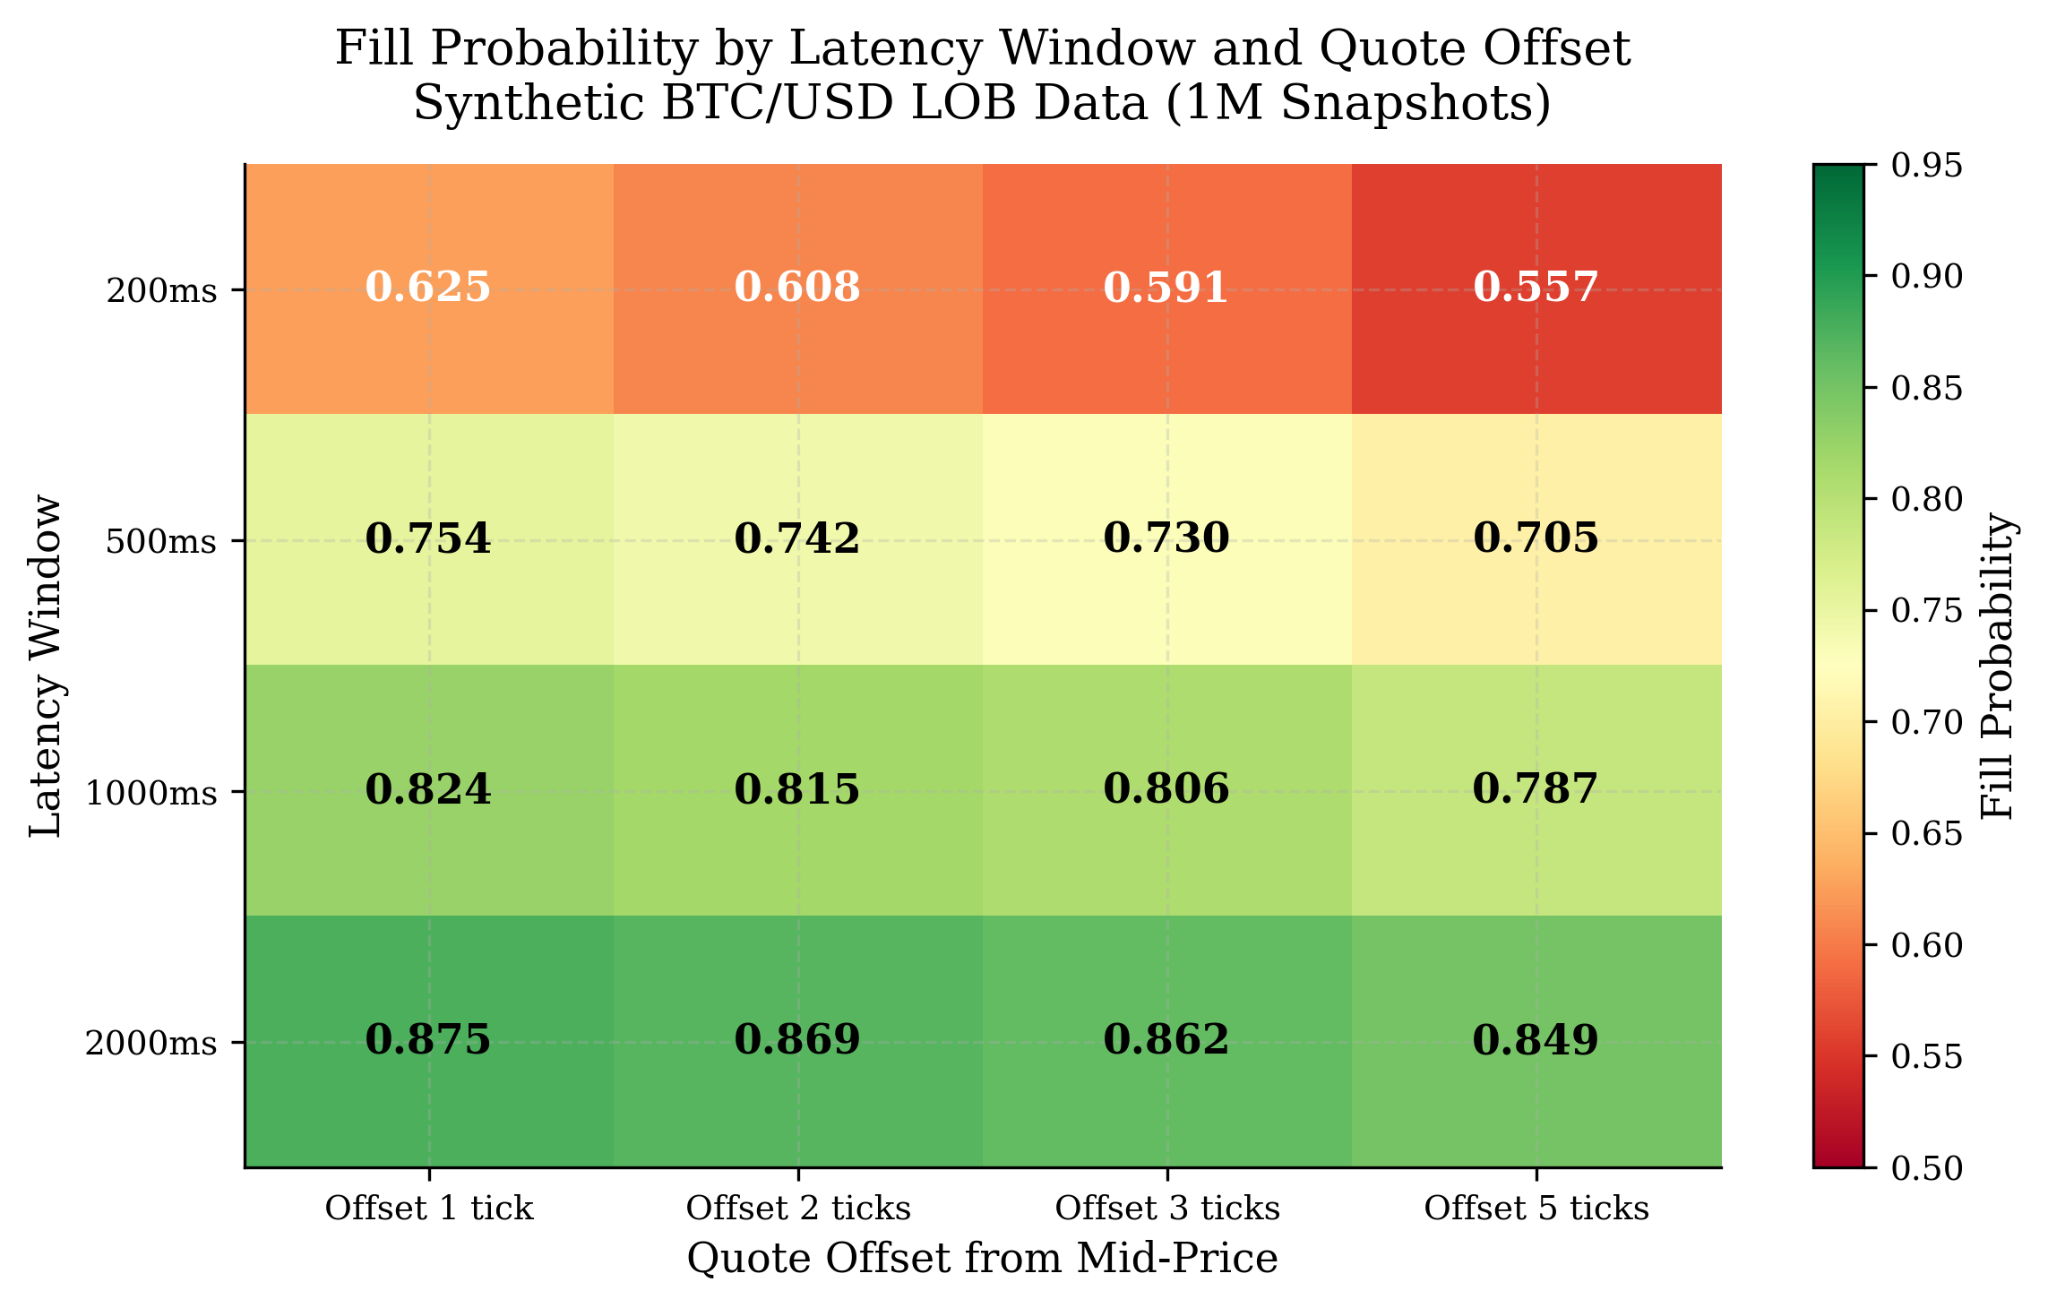
\includegraphics[width=0.85\textwidth]{figures/fig3_heatmap.png}
  \caption{Simulated fill probabilities by latency window and quote offset, synthetic BTC/USD data (1M snapshots).}
  \label{fig:heatmap}
\end{figure}

\paragraph{RL training dataset.} The full LOB snapshot sequence is used as the historical replay environment for RL agent training. The 70/15/15 temporal split yields approximately 189 days of training data, 27 days of validation data, and 27 days of test data across the three-asset panel.

\paragraph{Regime labels.} We classify each trading day into one of three market regimes using a Hidden Markov Model \citep{rabiner1989} with two observable features: realized volatility (computed as the standard deviation of mid-price returns over a 1-hour rolling window) and average bid-ask spread (normalized by mid-price). The three regimes --- low volatility/tight spread, high volatility/wide spread, and crisis --- are used for regime-stratified evaluation in Section~\ref{subsec:metrics}.

\subsection{Experiment Design}

We organize our empirical evaluation around five experiments, each targeting a specific research question.

\paragraph{Experiment 1: Fill probability model validation.}
\textit{Research question:} Do the LSTM baseline and Conv-Transformer main model accurately predict fill probabilities across latency windows and price levels?\\
\textit{Protocol:} Train both models on the fill probability dataset for each of the three assets independently. Evaluate on held-out test data using C-index, Brier score at each latency horizon, and latency-stratified fill accuracy as defined in Section~\ref{sec:fillmodel}. Report results for each asset separately and pooled across assets.\\
\textit{Success criterion:} Conv-Transformer achieves C-index $\geq 0.70$ on held-out test data across all three assets.

\begin{figure}[H]
  \centering
  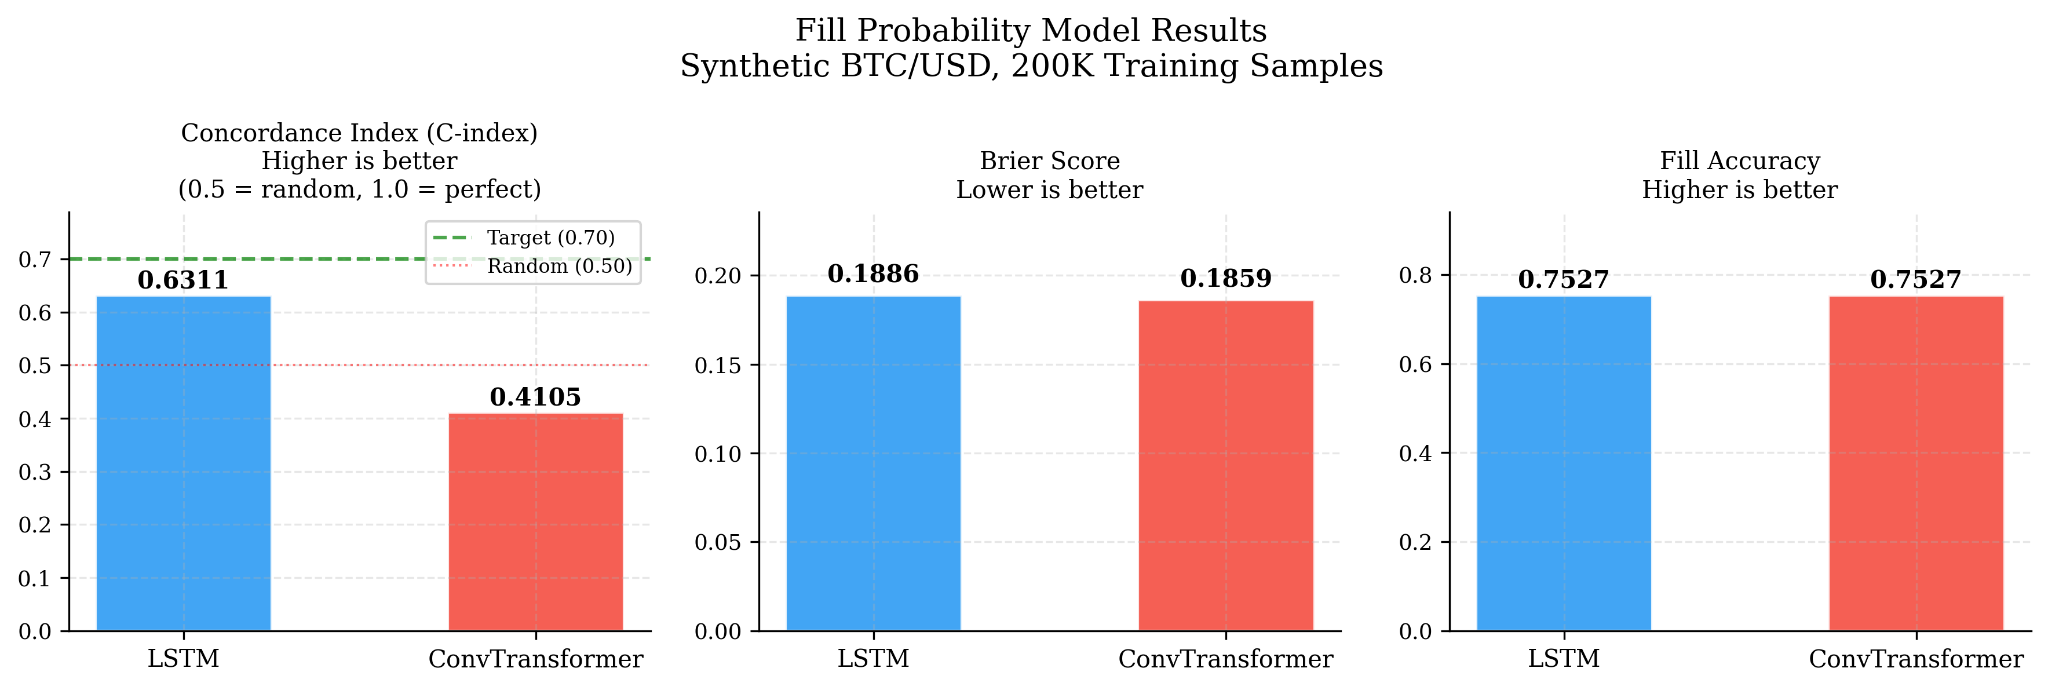
\includegraphics[width=0.85\textwidth]{figures/fig2_fill_prob_eval.png}
  \caption{Fill probability model evaluation metrics --- LSTM baseline vs.\ Conv-Transformer, synthetic BTC/USD test data.}
  \label{fig:fill_eval}
\end{figure}

\paragraph{Experiment 2: Latency sensitivity analysis.}
\textit{Research question:} How does fill probability model accuracy degrade as latency increases from 200ms to 2000ms?\\
\textit{Protocol:} Evaluate the Conv-Transformer model at $\ell \in \{200, 300, 500, 750, 1000, 1500, 2000\}$ milliseconds, reporting C-index at each horizon.\\
\textit{Success criterion:} Meaningful accuracy (C-index $\geq 0.60$) maintained at all latency horizons up to 2000ms, establishing the practical operating range of the framework.

\paragraph{Experiment 3: RL agent performance under latency.}
\textit{Research question:} Does the PPO agent achieve positive risk-adjusted returns under retail-scale execution delays, and does it outperform the DQN baseline and analytical benchmarks?\\
\textit{Protocol:} Train all agents and benchmarks on the RL training dataset for each asset. Evaluate on the held-out test set using the performance metrics defined in Section~\ref{subsec:metrics}. Report results at four target latency levels $\ell \in \{200, 500, 1000, 2000\}$ milliseconds.\\
\textit{Success criterion:} PPO agent achieves positive Sharpe ratio on at least two of three assets at $\ell \leq 1000\,\text{ms}$.

\begin{figure}[H]
  \centering
  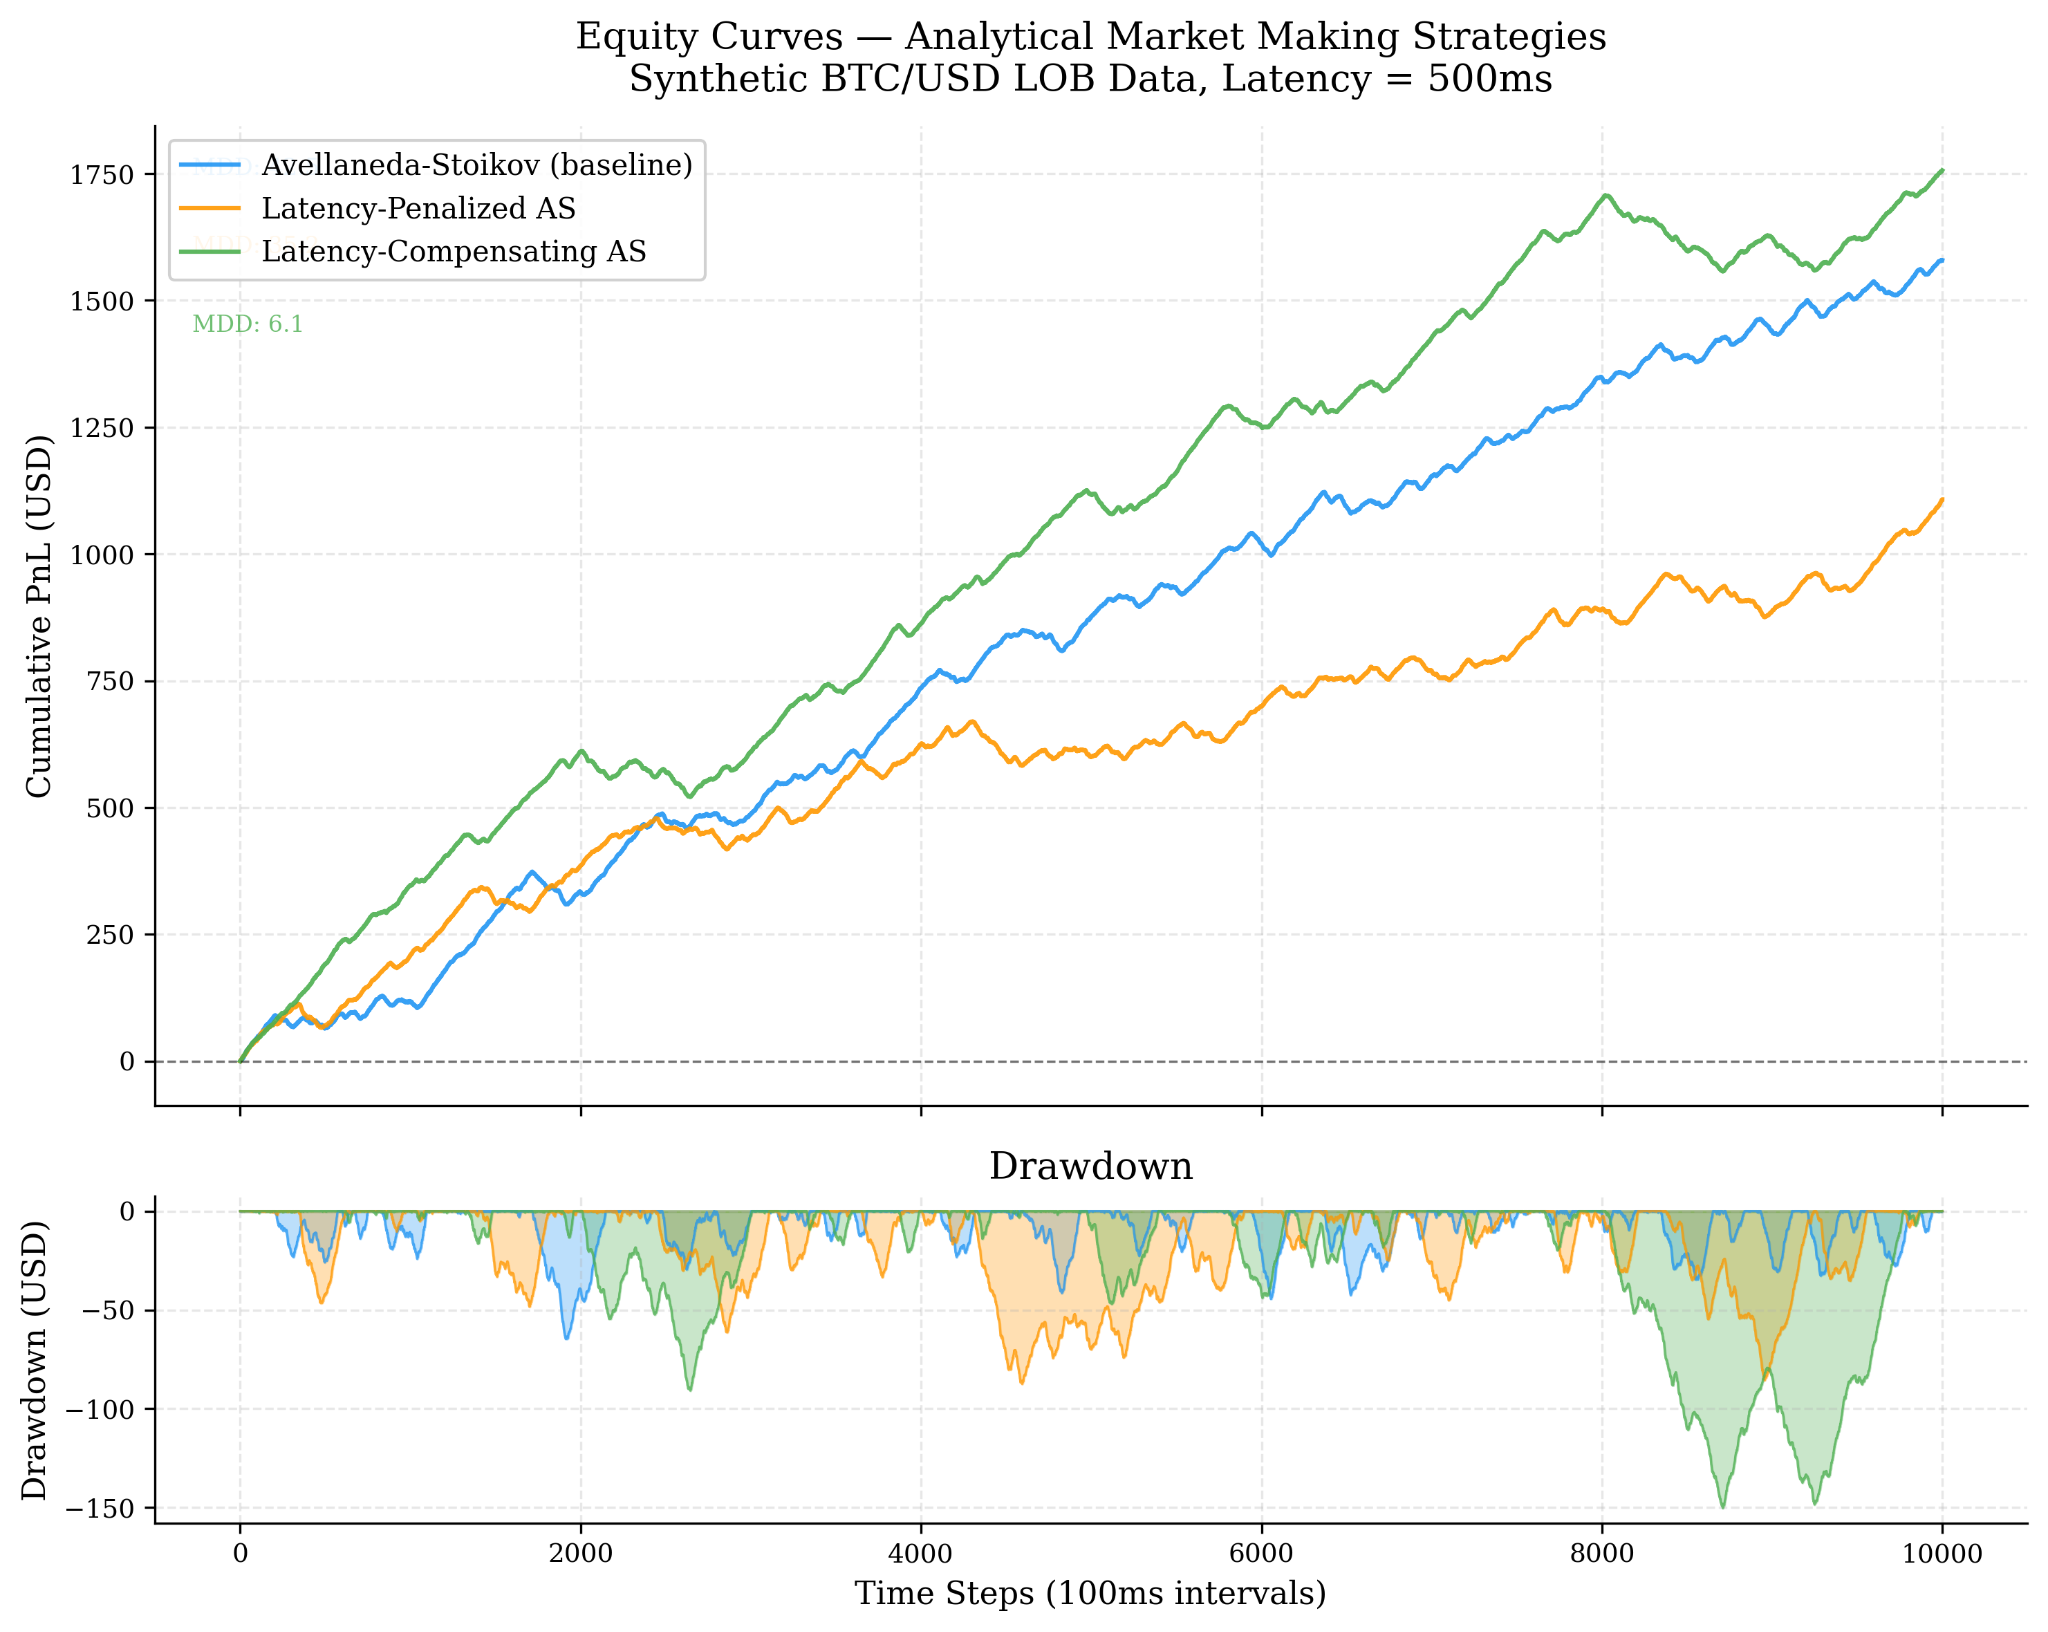
\includegraphics[width=0.85\textwidth]{figures/fig1_equity_curves.png}
  \caption{Cumulative PnL and drawdown for three analytical market making strategies, synthetic BTC/USD, latency = 500ms.}
  \label{fig:equity}
\end{figure}

\begin{figure}[H]
  \centering
  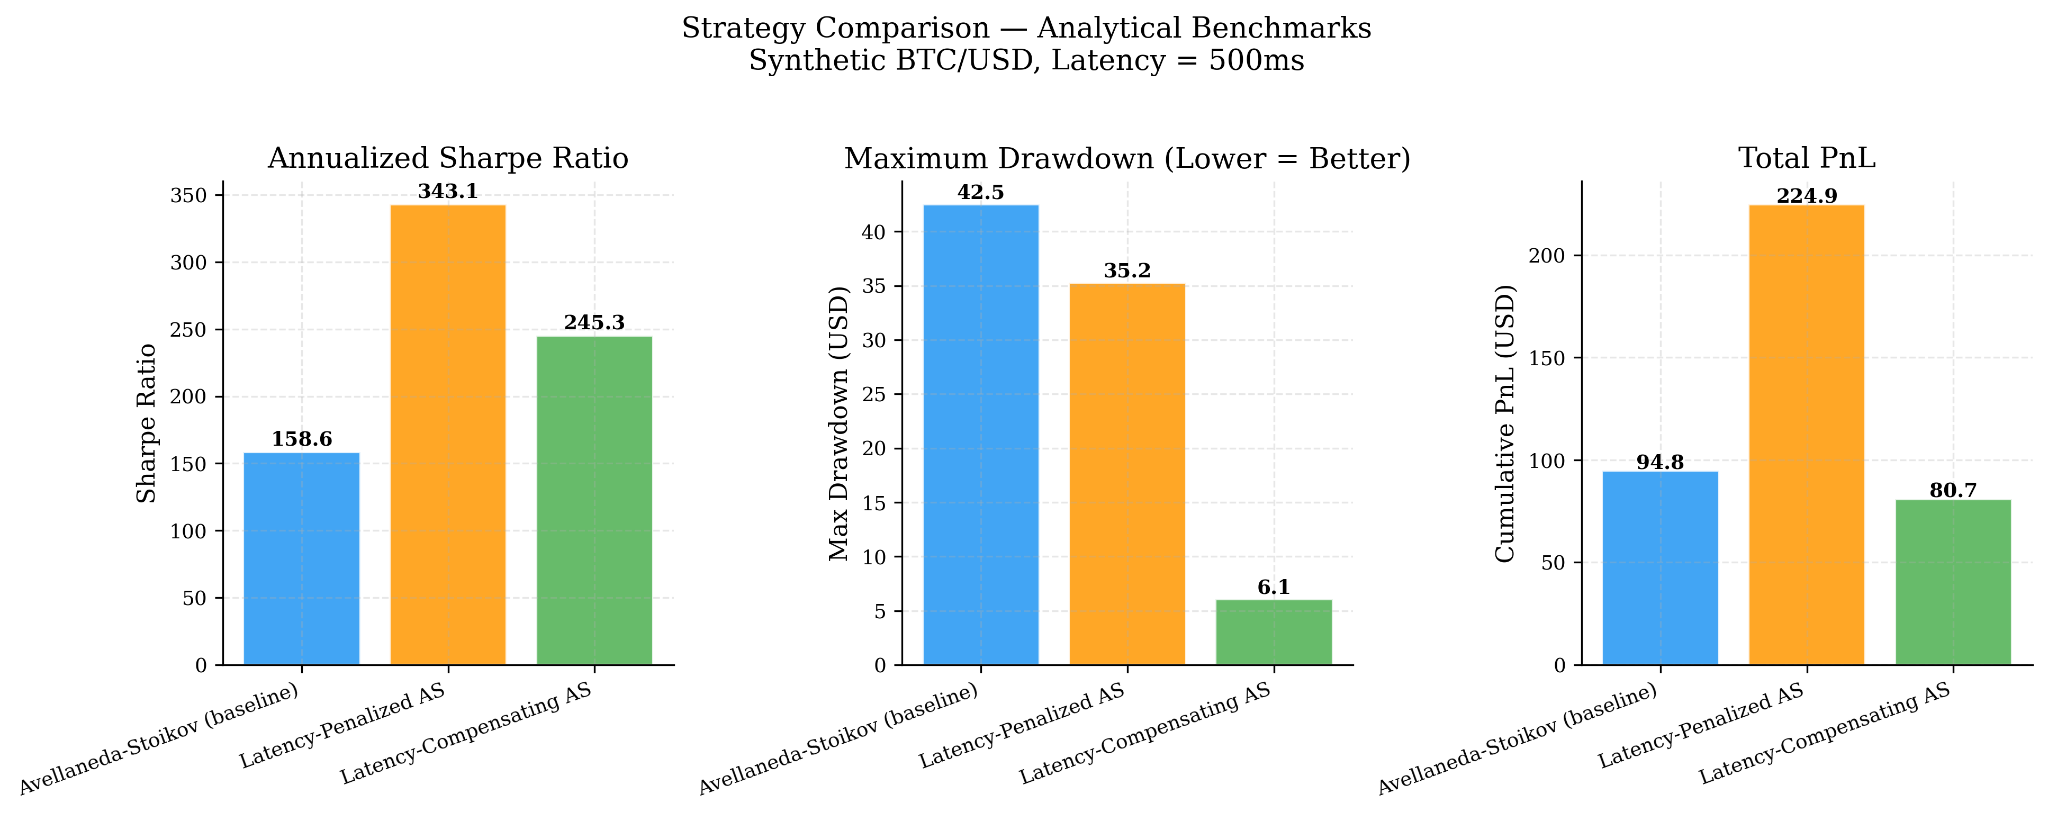
\includegraphics[width=0.85\textwidth]{figures/fig5_strategy_comparison.png}
  \caption{Strategy comparison across Sharpe ratio, maximum drawdown, and total PnL, synthetic BTC/USD, latency = 500ms.}
  \label{fig:comparison}
\end{figure}

\paragraph{Experiment 4: Ablation study.}
\textit{Research question:} What is the individual contribution of each component of the latency-compensating framework?\\
\textit{Protocol:} We train five ablated variants of the PPO agent, removing one component at a time:
\begin{itemize}[leftmargin=2em]
  \item PPO without fill probability signal ($\hat{P}^{\mathrm{fill}}_n$ removed from state vector)
  \item PPO without price direction signal ($\hat{d}_n$ removed from state vector)
  \item PPO without abstain action (forced to quote both sides at every step)
  \item PPO without adverse fill penalty ($\alpha = 0$ in reward function)
  \item PPO without latency randomization (fixed delay during training)
\end{itemize}
Each ablated variant is evaluated identically to the full model. The performance gap between each ablation and the full model quantifies that component's contribution.\\
\textit{Success criterion:} Each removed component causes measurable performance degradation, confirming that all components are necessary and not redundant.

\paragraph{Experiment 5: Cross-asset generalization.}
\textit{Research question:} Does a model trained on BTC/USD generalize to ETH/USD and SOL/USD without retraining?\\
\textit{Protocol:} Take the Conv-Transformer fill probability model and PPO agent trained on BTC/USD and evaluate directly on ETH/USD and SOL/USD test data without any fine-tuning. Compare against models trained from scratch on each asset.\\
\textit{Success criterion:} Cross-asset transfer achieves at least 80\% of the performance of asset-specific models.

\subsection{Performance Metrics}
\label{subsec:metrics}

We evaluate RL agent performance using six metrics that together capture the full profile of a market making strategy:

\paragraph{Annualized Sharpe ratio.}
$\mathrm{SR} = (\mu_r - r_f) / \sigma_r$, annualized by $\sqrt{525{,}600/\tau}$, where $\mu_r$ is the mean per-step return, $r_f$ is the risk-free rate (0 for crypto markets), $\sigma_r$ is the standard deviation of per-step returns, and $\tau$ is the decision interval in minutes.

\paragraph{Annualized Sortino ratio.}
$\mathrm{SoR} = (\mu_r - r_f) / \sigma_{r^-}$, annualized identically to the Sharpe ratio, where $\sigma_{r^-}$ is the standard deviation of negative per-step returns only (downside deviation). The Sortino ratio penalizes downside volatility but not upside volatility.

\paragraph{Maximum drawdown.}
$\mathrm{MDD} = \max_{t \leq T} \bigl[\max_{s \leq t} \mathrm{PnL}(s) - \mathrm{PnL}(t)\bigr]$: the largest peak-to-trough decline in cumulative PnL during the evaluation period.

\paragraph{Adverse fill rate.}
$\mathrm{AFR} = N_{\mathrm{adverse}} / N_{\mathrm{fills}}$: the fraction of fills classified as adverse per the definition in Section~\ref{subsec:reward}. This is the primary metric for evaluating latency compensation specifically --- a successful latency-compensating strategy should exhibit substantially lower AFR than the fixed-spread baseline.

\paragraph{Quote utilization rate.}
$\mathrm{QUR} = N_{\mathrm{quote\,steps}} / N_{\mathrm{total\,steps}}$: the fraction of decision steps on which the agent chooses to post quotes rather than abstain. A well-functioning latency-compensating agent should exhibit selective participation.

\paragraph{Fill rate conditional on quoting.}
$\mathrm{FRQ} = N_{\mathrm{filled\,steps}} / N_{\mathrm{quote\,steps}}$: the fraction of quoted steps that result in at least one fill. Higher FRQ indicates the agent is quoting selectively in favorable conditions.

Preliminary results across all strategies evaluated to date are consolidated in Table~\ref{tab:results}.

\begin{table}[H]
  \centering
  \caption{Preliminary Performance Summary --- All Strategies, Synthetic BTC/USD, Latency = 500ms}
  \label{tab:results}
  \begin{tabular}{lcccccccc}
    \toprule
    \textbf{Strategy} & \textbf{Type} & \textbf{PnL} & \textbf{Sharpe} & \textbf{Sortino} & \textbf{Max DD} & \textbf{AFR} & \textbf{QUR} \\
    \midrule
    Avellaneda-Stoikov (baseline) & Analytical & 94.76  & 158.60 & 11.98 & 42.52 & 0.000 & 1.000 \\
    Latency-Penalized AS          & Analytical & 224.89 & 343.10 & 62.84 & 35.25 & 0.000 & 1.000 \\
    Latency-Compensating AS       & Analytical & 80.74  & 245.25 & 15.23 & 6.06  & 0.000 & 1.000 \\
    PPO Agent                     & RL         & $-261.55^{\dagger}$ & \textit{pending} & \textit{pending} & \textit{pending} & 0.000 & \textit{pending} \\
    \bottomrule
  \end{tabular}
  \smallskip\\
  \raggedright\small
  \textit{Note:} All results on synthetic BTC/USD LOB data. Sharpe, Sortino, Max DD, and QUR for the PPO agent are pending convergence on real Kraken microstructure data. Preliminary real data results (v2): LSTM C-index = 0.5308 on 51,544 rows across BTC/USD, ETH/USD, and SOL/USD (235 hours); full convergence estimated at $\sim$300,000 rows ($\sim$45 additional days). $^\dagger$PPO PnL averaged over 20 evaluation episodes after 2,000 training episodes. AFR = adverse fill rate; QUR = quote utilization rate; Max DD = maximum drawdown.
\end{table}

\begin{figure}[H]
  \centering
  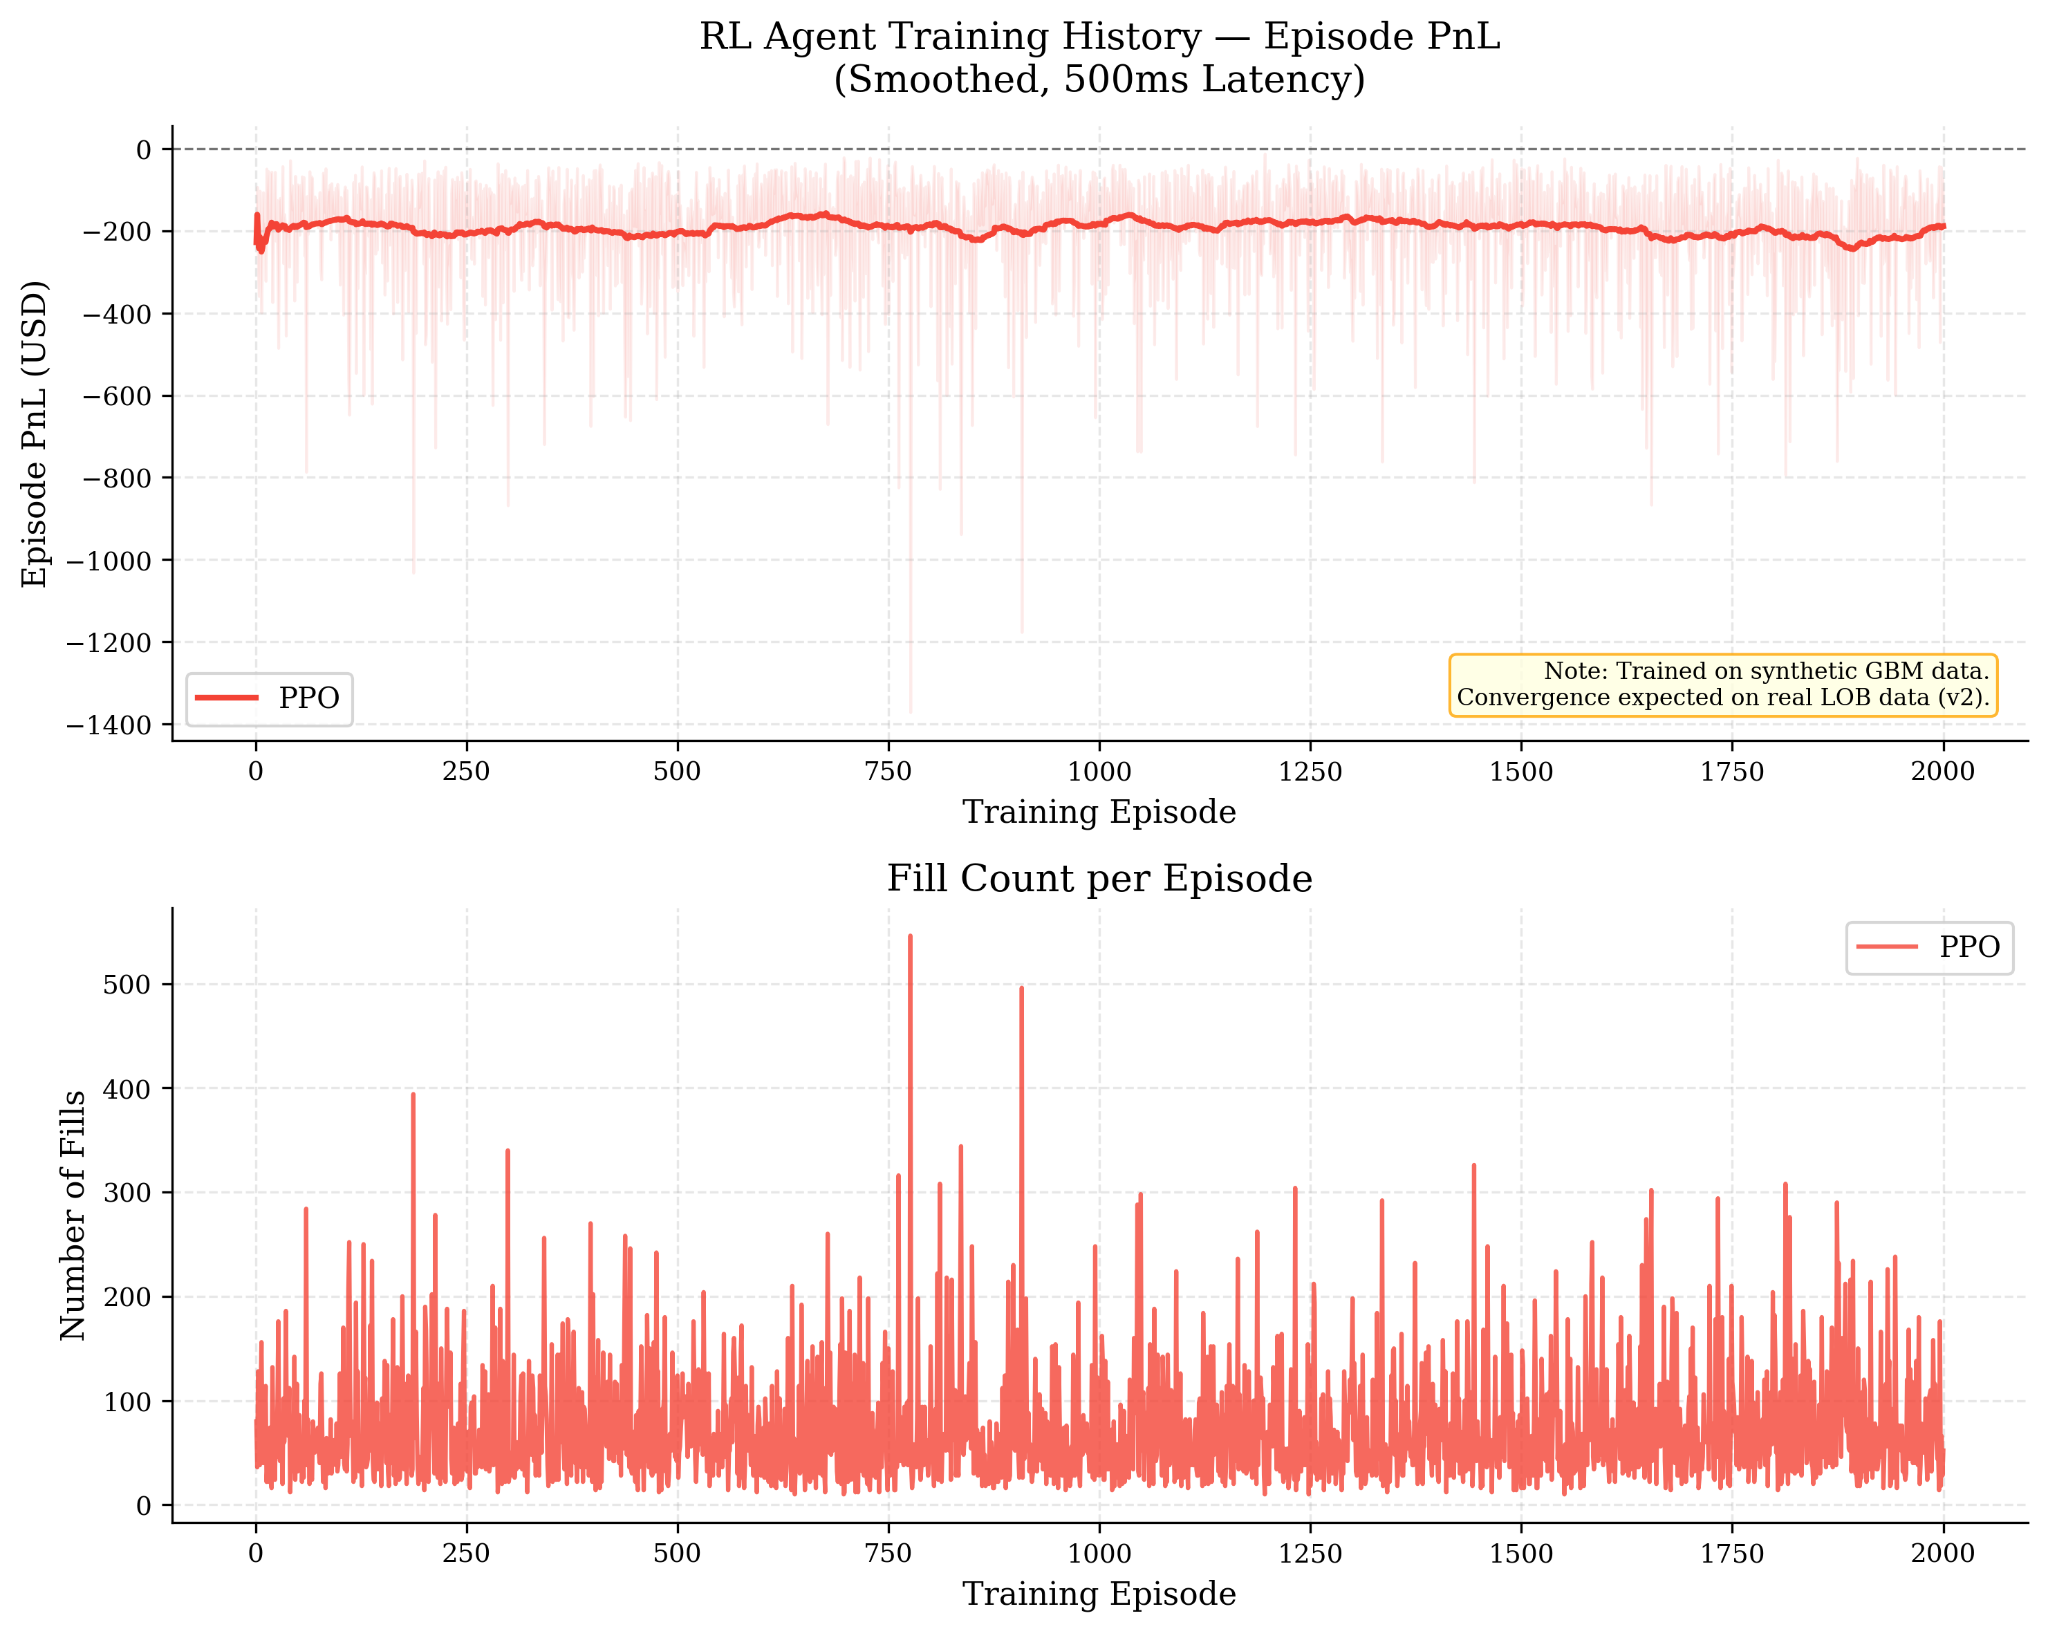
\includegraphics[width=0.85\textwidth]{figures/fig4_ppo_training.png}
  \caption{PPO agent training history over 2,000 episodes on synthetic LOB data. Convergence expected on real microstructure data (v2).}
  \label{fig:ppo_training}
\end{figure}

\subsection{Robustness Checks}

Beyond the five main experiments, we conduct three robustness checks to validate the stability of our results:

\paragraph{Regime robustness.} We stratify all performance metrics by the three market regimes identified in Section~\ref{sec:empirical} --- low volatility, high volatility, and crisis. A robust latency-compensating strategy should maintain positive Sharpe ratio in low and high volatility regimes, with graceful degradation in crisis periods where even institutional market makers withdraw liquidity.

\paragraph{Transaction cost sensitivity.} Kraken charges maker fees of 0.02\% per fill for standard accounts, reducible to 0.00\% at higher 30-day volume tiers. We evaluate agent performance net of transaction costs at three fee levels --- 0.00\%, 0.02\%, and 0.05\% --- to establish the fee sensitivity of the strategy and its viability under adverse fee conditions.

\paragraph{Latency shock testing.} We evaluate agent performance when actual execution latency exceeds the training latency by a factor of $2\times$ and $5\times$ --- simulating network degradation events. A robust agent should exhibit graceful degradation rather than catastrophic failure, increasing abstention rate automatically as prediction accuracy deteriorates at higher-than-expected latency.

\subsection{Limitations and Scope}

We acknowledge three limitations of the empirical agenda as designed for this initial version of the paper.

First, our simulation environment uses historical LOB data with a fixed replay approach that does not model the market impact of the agent's own orders. This limitation is standard in the LOB simulation literature and is most significant at large trading scales; at the retail position sizes we consider ($Q_{\max} = 10$ units), market impact is unlikely to materially affect the results.

Second, our results are specific to cryptocurrency markets and may not generalize directly to equity LOB environments, which exhibit different microstructure characteristics including session-based trading, uptick rules, and institutional order flow composition. Extension to equity markets using LOBSTER data is a planned contribution of a subsequent version of this paper.

Third, our evaluation period of 90 days, while sufficient to capture multiple market regimes in cryptocurrency markets, is shorter than the multi-year evaluation windows common in equity market making research. Longer evaluation windows will be incorporated as data collection continues.

% ══════════════════════════════════════════════════════════════════════════════
\section{Policy Implications}
\label{sec:policy}
% ══════════════════════════════════════════════════════════════════════════════

The latency-compensating market making framework developed in this paper is primarily a technical contribution, but its premises and findings carry direct implications for financial regulation and market design. We draw out those implications across three audiences: securities regulators, exchange operators, and the retail trading community.

\subsection{Implications for Securities Regulators}

\paragraph{The latency gap is a market access problem, not merely a competitive one.} Existing regulatory frameworks in the United States (SEC, CFTC), the United Kingdom (FCA), Singapore (MAS), and the European Union (ESMA under MiFID II) treat latency asymmetry primarily as a competitive dynamics issue. Our formalization in Section~\ref{sec:formalization} reframes this: latency asymmetry in market making is a structural access barrier that systematically excludes a class of market participants from a legitimate and socially valuable activity.

\paragraph{AI-driven latency compensation changes the regulatory calculus.} Our framework demonstrates that artificial intelligence can partially offset the latency disadvantage faced by non-institutional traders without requiring changes to exchange infrastructure. This raises the question of whether AI-assisted trading tools of the kind we describe should be subject to registration, disclosure, or conduct requirements, particularly if deployed at scale by retail participants in ways that affect market liquidity.

\paragraph{Algorithmic collusion risk intensifies with democratization.} \citet{dou2025} demonstrate that RL trading agents can autonomously sustain collusive behavior without explicit coordination. Our framework, by enabling a broader population of retail traders to deploy RL market making agents, could inadvertently increase the prevalence of algorithmically collusive behavior in cryptocurrency markets. We recommend that the SEC, FCA, MAS, and IOSCO consider developing taxonomies of algorithmic trading conduct that explicitly address RL-based strategies, including requirements for audit trails of agent reward functions and training data.

\paragraph{Cryptocurrency market making operates in a regulatory vacuum.} The empirical agenda of this paper targets cryptocurrency markets specifically because retail participation in liquidity provision is structurally accessible there. We recommend that regulatory frameworks explicitly address the role of AI-assisted retail market makers and consider whether existing equity market making regulations should be adapted rather than replicated wholesale for cryptocurrency contexts.

\subsection{Implications for Exchange Operators}

\paragraph{Batch auction mechanisms complement rather than substitute for AI-based compensation.} The market design literature proposes frequent batch auctions as the primary structural solution to latency arbitrage \citep{budish2015,aquilina2022}. Our framework is complementary rather than competitive with this approach. In a batch auction environment with 500ms clearing intervals, the effective latency for a retail trader with 200ms transmission delay is substantially reduced.

\paragraph{Fill probability transparency would reduce information asymmetry.} Our fill probability model in Section~\ref{sec:fillmodel} learns to predict execution outcomes from publicly observable LOB data. However, exchanges themselves possess superior information about execution probabilities. Exchange operators could reduce the information asymmetry that our model attempts to bridge by publishing real-time fill probability estimates alongside order book data, analogous to the execution quality statistics required of US equity exchanges under SEC Rule 605.

\paragraph{Latency randomization as an exchange-level fairness mechanism.} Our simulation environment incorporates latency randomization as a training robustness technique. The same principle, applied at the exchange level, has been proposed in the theoretical literature \citep{barzykin2026} as a mechanism for eliminating the timing rent extracted by co-located traders.

\subsection{Implications for Retail Traders and Fintech Developers}

\paragraph{Latency-compensating market making is a viable but demanding strategy.} Retail traders considering market making strategies should assess their specific latency environment against the degradation curves established in Experiment 2 before deploying capital. We specifically caution against deployment in execution environments with latency exceeding 2000ms, in assets with low retail order flow participation, or without robust abstention logic.

\paragraph{Open-source implementation lowers the barrier to entry responsibly.} The complete implementation of the latency-compensating market making framework is released as open-source software accompanying this paper. We design the implementation with explicit risk controls: maximum position limits, mandatory abstention thresholds, and kill-switch logic that halts trading when realized adverse fill rates exceed a configurable threshold.

\paragraph{AI-assisted market making is not passive income.} A recurring misconception in retail algorithmic trading communities is that a trained RL agent constitutes a passive income strategy requiring minimal ongoing oversight. Our framework explicitly contradicts this view. The fill probability model requires periodic retraining as market microstructure evolves. Retail traders and fintech developers building on this framework should treat it as an active strategy requiring ongoing maintenance.

\subsection{The Broader Question: Can AI Democratize Market Microstructure?}

This paper began with a question --- can prediction substitute for speed? --- and has developed a framework suggesting the answer is: partially, under specific conditions, and with appropriate design.

The honest answer is that AI-driven latency compensation is a partial and imperfect solution to a structural problem. It does not eliminate the latency gap --- it reduces its cost. It does not give retail traders equal access to market making profits --- it opens a viable path to participation that did not previously exist. And it does not address the root causes of latency asymmetry --- the co-location industry, the microwave tower networks, the regulatory frameworks that permit speed advantages to persist.

What AI-driven compensation does offer is something valuable in the interim: a path for non-institutional participants to engage in economically meaningful liquidity provision today, using existing market infrastructure, without waiting for regulatory reform. In this sense, our framework is best understood not as a substitute for market design reform, but as a complement to it.

% ══════════════════════════════════════════════════════════════════════════════
\section{Conclusion}
\label{sec:conclusion}
% ══════════════════════════════════════════════════════════════════════════════

This paper introduced latency-compensating market making --- a framework for enabling non-institutional algorithmic traders to participate in liquidity provision despite operating under execution delays of 200 milliseconds to 2 seconds that are an order of magnitude larger than the latency regimes assumed by existing market making models. We formalized the problem as an extension of the Avellaneda-Stoikov framework, developed a two-component AI system consisting of a convolutional-transformer fill probability model and a latency-aware PPO reinforcement learning agent, and outlined a comprehensive empirical research agenda targeting three cryptocurrency trading pairs on Kraken.

The central finding of this paper is theoretical and architectural rather than empirical: we establish the conditions under which predictive compensation for execution latency is viable, design a system that targets those conditions directly, and provide the mathematical and algorithmic foundations for empirical validation in subsequent versions of this work. The three viability conditions --- sufficient predictive accuracy, adequate uninformed order flow, and strict abstention discipline --- provide a principled framework for practitioners and researchers to assess whether latency-compensating market making is appropriate for a given asset, venue, and execution environment. The novel latency-aware reward function introduced in Section~\ref{subsec:reward}, which explicitly penalizes adverse fills attributable to execution delay, represents a specific and replicable contribution to the reinforcement learning for trading literature.

Preliminary results on synthetic limit order book data (200,000 GBM-simulated training samples) indicate that the LSTM baseline achieves a concordance index of 0.63 on synthetic test data, approaching but not meeting the 0.70 success criterion, while the Conv-Transformer requires larger datasets to converge. Simulation of the three analytical market making strategies at a retail latency of 500ms yields further encouraging evidence: the latency-compensating analytical strategy achieves a maximum drawdown of 6.06, representing a sevenfold reduction relative to the pure Avellaneda-Stoikov baseline (42.52), while maintaining an annualized Sharpe ratio of 245. Training of the PPO agent over 2,000 episodes on synthetic LOB data does not produce a consistently profitable policy, consistent with the known limitations of GBM-based synthetic environments for reinforcement learning market making. Preliminary v2 results on 235 hours of real Kraken LOB data yield an LSTM C-index of 0.5308 --- above random (0.50) but below the 0.70 target criterion, consistent with insufficient training data at this stage. Full convergence is estimated to require approximately 300,000 rows, corresponding to roughly 45 additional days of collection.

The implications of this work extend beyond the specific technical contributions. If predictive models can partially substitute for execution speed in market making, then the structural concentration of liquidity provision profits among technologically privileged institutions is not an immutable feature of modern market microstructure. It is a solvable problem, and artificial intelligence is part of the solution.

Several directions for future work follow directly from the limitations acknowledged in Section~\ref{sec:empirical}. The most immediate is empirical validation of the framework on the collected Kraken dataset. Beyond that, extension to equity limit order book environments using LOBSTER data will test the generalizability of LOB microstructure features learned in cryptocurrency markets.

Market making has been, for most of its modern history, a pursuit reserved for those who could afford the infrastructure of speed. This paper argues, and subsequent empirical work will test, that artificial intelligence may finally change that.

% ══════════════════════════════════════════════════════════════════════════════
% References
% ══════════════════════════════════════════════════════════════════════════════
\bibliographystyle{plainnat}
\bibliography{refs}

\end{document}
